\documentclass[tikz, border=10pt]{standalone}
\usetikzlibrary{shapes.geometric, arrows.meta, positioning}

\usepackage{amssymb}
\usepackage[fleqn,reqno]{amsmath}
\usepackage{mathtools}

\begin{document}

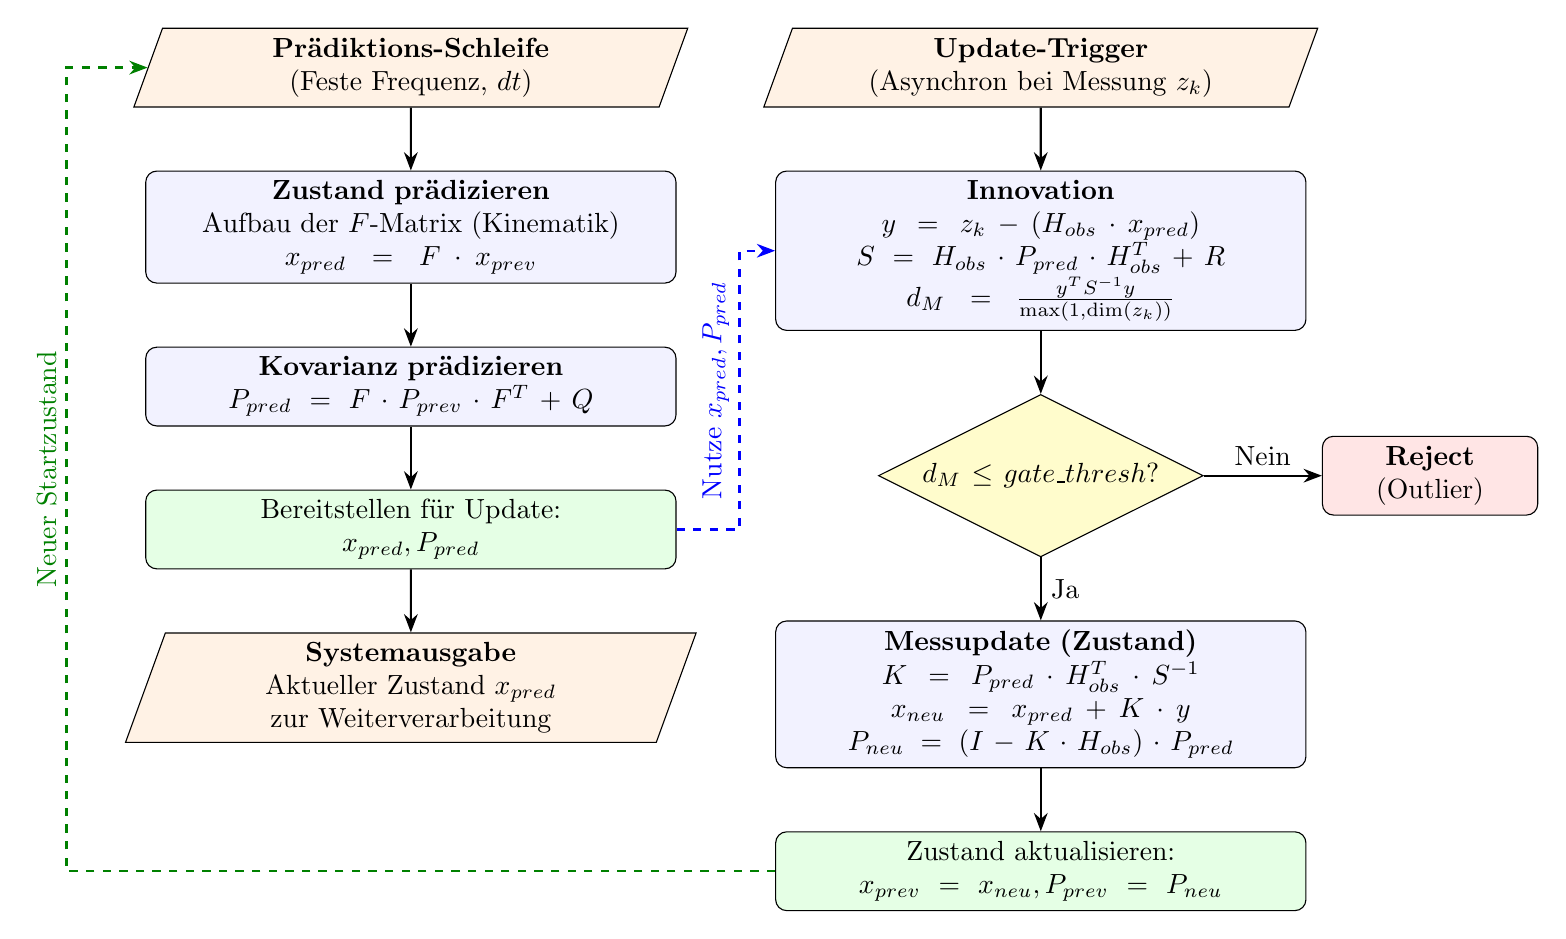
\begin{tikzpicture}[
    node distance=0.8cm and 1cm,
    auto,
    block/.style={rectangle, draw, fill=blue!5, text width=6.5cm, align=center, rounded corners, minimum height=1cm},
    io/.style={trapezium, trapezium left angle=70, trapezium right angle=110, draw, fill=orange!10, text width=6cm, align=center, minimum height=1cm},
    decision/.style={diamond, aspect=2, draw, fill=yellow!20, text width=3.5cm, align=center, inner sep=0pt},
    reject/.style={rectangle, draw, fill=red!10, text width=2.5cm, align=center, rounded corners, minimum height=1cm},
    line/.style={draw, -Stealth, thick}
]

% --- PRÄDIKTIONS-STRANG ---
\node [io] (timer) at (0,0) {
    \textbf{Prädiktions-Schleife} \\ 
    (Feste Frequenz, $dt$)
};

\node [block, below=of timer] (pred_state) {
    \textbf{Zustand prädizieren} \\
    Aufbau der $F$-Matrix (Kinematik) \\
    $x_{pred} = F \cdot x_{prev}$
};

\node [block, below=of pred_state] (pred_cov) {
    \textbf{Kovarianz prädizieren} \\
    $P_{pred} = F \cdot P_{prev} \cdot F^T + Q$
};

\node [block, below=of pred_cov, fill=green!10] (save_pred) {
    Bereitstellen für Update: \\ $x_{pred}, P_{pred}$
};

\node [io, below=of save_pred] (sys_out) {
    \textbf{Systemausgabe} \\
    Aktueller Zustand $x_{pred}$ \\ zur Weiterverarbeitung
};

% --- UPDATE-STRANG ---
\node [io] (meas) at (8,0) {
    \textbf{Update-Trigger} \\ 
    (Asynchron bei Messung $z_k$)
};

\node [block, below=of meas] (innov) {
    \textbf{Innovation} \\
    $y = z_k - (H_{obs} \cdot x_{pred})$ \\
    $S = H_{obs} \cdot P_{pred} \cdot H_{obs}^T + R$ \\
    $d_M = \frac{y^T S^{-1} y}{\max(1, \dim(z_k))}$
};

\node [decision, below=of innov] (maha) {
    $d_M \le gate\_thresh$?
};

\node [reject, right=1.5cm of maha] (reject) {
    \textbf{Reject} \\ (Outlier)
};

\node [block, below=0.8cm of maha] (update) {
    \textbf{Messupdate (Zustand)} \\
    $K = P_{pred} \cdot H_{obs}^T \cdot S^{-1}$ \\
    $x_{neu} = x_{pred} + K \cdot y$ \\
    $P_{neu} = (I - K \cdot H_{obs}) \cdot P_{pred}$
};

\node [block, below=of update, fill=green!10] (save_upd) {
    Zustand aktualisieren: \\ $x_{prev} = x_{neu}, P_{prev} = P_{neu}$
};

% --- PFEILE ---
\path [line] (timer) -- (pred_state);
\path [line] (pred_state) -- (pred_cov);
\path [line] (pred_cov) -- (save_pred);
\path [line] (save_pred) -- (sys_out);

\path [line] (meas) -- (innov);
\path [line] (innov) -- (maha);
\path [line] (maha) -- node[above] {Nein} (reject);
\path [line] (maha) -- node[right] {Ja} (update);
\path [line] (update) -- (save_upd);

\draw [line, dashed, blue] (save_pred.east) -- ++(0.8,0) |- (innov.west) node[pos=0.25, above, rotate=90] {Nutze $x_{pred}, P_{pred}$};
\draw [line, dashed, green!50!black] (save_upd.west) -- ++(-9,0) |- (timer.west) node[pos=0.25, above, rotate=90] {Neuer Startzustand};

\end{tikzpicture}

\end{document}